% AAAI-27 anonymous submission draft (parallel to doc/AAAI_SUBMISSION_DRAFT.md)
% ---------------------------------------------------------------------------
% OVERLEAF SETUP
% 1. New Project -> Upload Project -> upload the whole AuthorKit27 folder, OR
%    upload this .tex into a project that already contains aaai2027.sty / .bst
% 2. Menu -> Main document -> AAAI_SUBMISSION_DRAFT.tex
% 3. Compiler: pdfLaTeX ; Recompile
% 4. Paste sections from this file; keep a SINGLE .tex (AAAI rule)
% ---------------------------------------------------------------------------
% Page budget: <=7 content pages; pages 8--9 references only.
% Blind: no real names/affiliations/acknowledgments for review.
% ---------------------------------------------------------------------------

\documentclass[letterpaper]{article} % DO NOT CHANGE THIS
\usepackage[submission]{aaai2027}  % DO NOT CHANGE THIS
% Fonts are loaded by aaai2027.sty --- do NOT add times/helvet/courier packages.
\usepackage[hyphens]{url}  % DO NOT CHANGE THIS
\usepackage{graphicx} % DO NOT CHANGE THIS
\urlstyle{rm} % DO NOT CHANGE THIS
\def\UrlFont{\rm}  % DO NOT CHANGE THIS
\usepackage{natbib}  % DO NOT CHANGE THIS AND DO NOT ADD ANY OPTIONS TO IT
\usepackage{caption} % DO NOT CHANGE THIS AND DO NOT ADD ANY OPTIONS TO IT
\frenchspacing  % DO NOT CHANGE THIS
\usepackage{booktabs}
\usepackage{amsmath}
\graphicspath{{figures/}{../doc/figures/}{./}}

\pdfinfo{
/TemplateVersion (2027.1)
}

% Number sections for AAAI main-track readability
\setcounter{secnumdepth}{2}

% Title Case (Chicago / AAAI): capitalize major words
\title{Dual-Expert Keys for Reducing False-Positive Retrieval in Lifelong Vision--Language Model Editing}

% Anonymous submission (required for review)
\author{
    Anonymous Submission
}
\affiliations{
    % Leave empty for blind review
}

\begin{document}

\maketitle

\begin{abstract}
Lifelong vision--language editors can look correct on the image they were edited for, then still emit the new fact when the scene is only visually related. In our probes this is usually not soft overwrite of the base model. It is false-positive retrieval (false-cross): weak visual keys make a different stored edit look good enough to retrieve, so the wrong expert fires. We address it in two steps. Dual-Expert Keys let an edit fire only when the visual match and the prompt-key match both pass. Separately, adversarial visual binding training attaches each edit to its correct image and lowers expert activation when the image is swapped or a hard negative. On VLKEB-based adversarial grounding probes, Dual-Expert Keys cut swap false-positive retrieval rate from 96\% to 46\% over five seeds and keep reliability near 94\%. Adversarial visual binding training complements Dual-Expert Keys by stabilizing edit--image binding under these adversarial probes. Against Fine-tuning, MEND-VL, and SERAC-VL on the same probes, we keep high reliability while directly reducing the wrong-expert retrieval rate.
\end{abstract}

\section{Introduction}
Large vision--language models (VLMs) now answer questions about photographs, documents, and everyday scenes, and they are often treated as soft knowledge bases in interactive systems~\citep{li2023blip2}.
Facts encoded in these models drift: places change names, entities are mislabeled, and new visual knowledge appears after pre-training ends.
Full fine-tuning is costly and can disturb unrelated skills, so \emph{model editing} has emerged as a practical alternative---apply a local update that corrects a target fact while preserving behaviour elsewhere~\citep{mitchell2022mend,mitchell2022serac,cheng2023mmedit}.
Multimodal benchmarks such as MMEdit and VLKEB standardize this goal around reliability, generality, and locality~\citep{cheng2023mmedit,huang2024vlkeb}.
When edits must arrive one after another, the problem becomes \emph{lifelong} editing: each new fact joins a growing set of updates that must remain available without overwriting earlier ones~\citep{chen2025liveedit}.

Retrieval- and mixture-of-experts (MoE) editors are a natural fit for that setting.
They store each edit as an expert (or memory entry) and, at test time, retrieve which expert(s) to inject for a query~\citep{mitchell2022serac,chen2025liveedit}.
On the image used for the edit, these systems can look excellent: reliability often sits in the low-to-mid 90s.
The harder question is whether the edit is \emph{visually grounded}.
Consider a city-entity edit with prompt $p$ (``What city in Illinois is depicted in the image?'') and target answer ``Kankakee.''
With the edited photograph, the post-edit model answers correctly.
With the \emph{same} prompt but a swapped skyline or a confusable hard-negative scene, a retrieval editor can still surface ``Kankakee'' (Figure~\ref{fig:teaser}).
That behaviour is especially damaging in lifelong pools: the more experts accumulate, the more chances a weak visual key has to match the wrong past edit.

\begin{figure}[t]
\centering
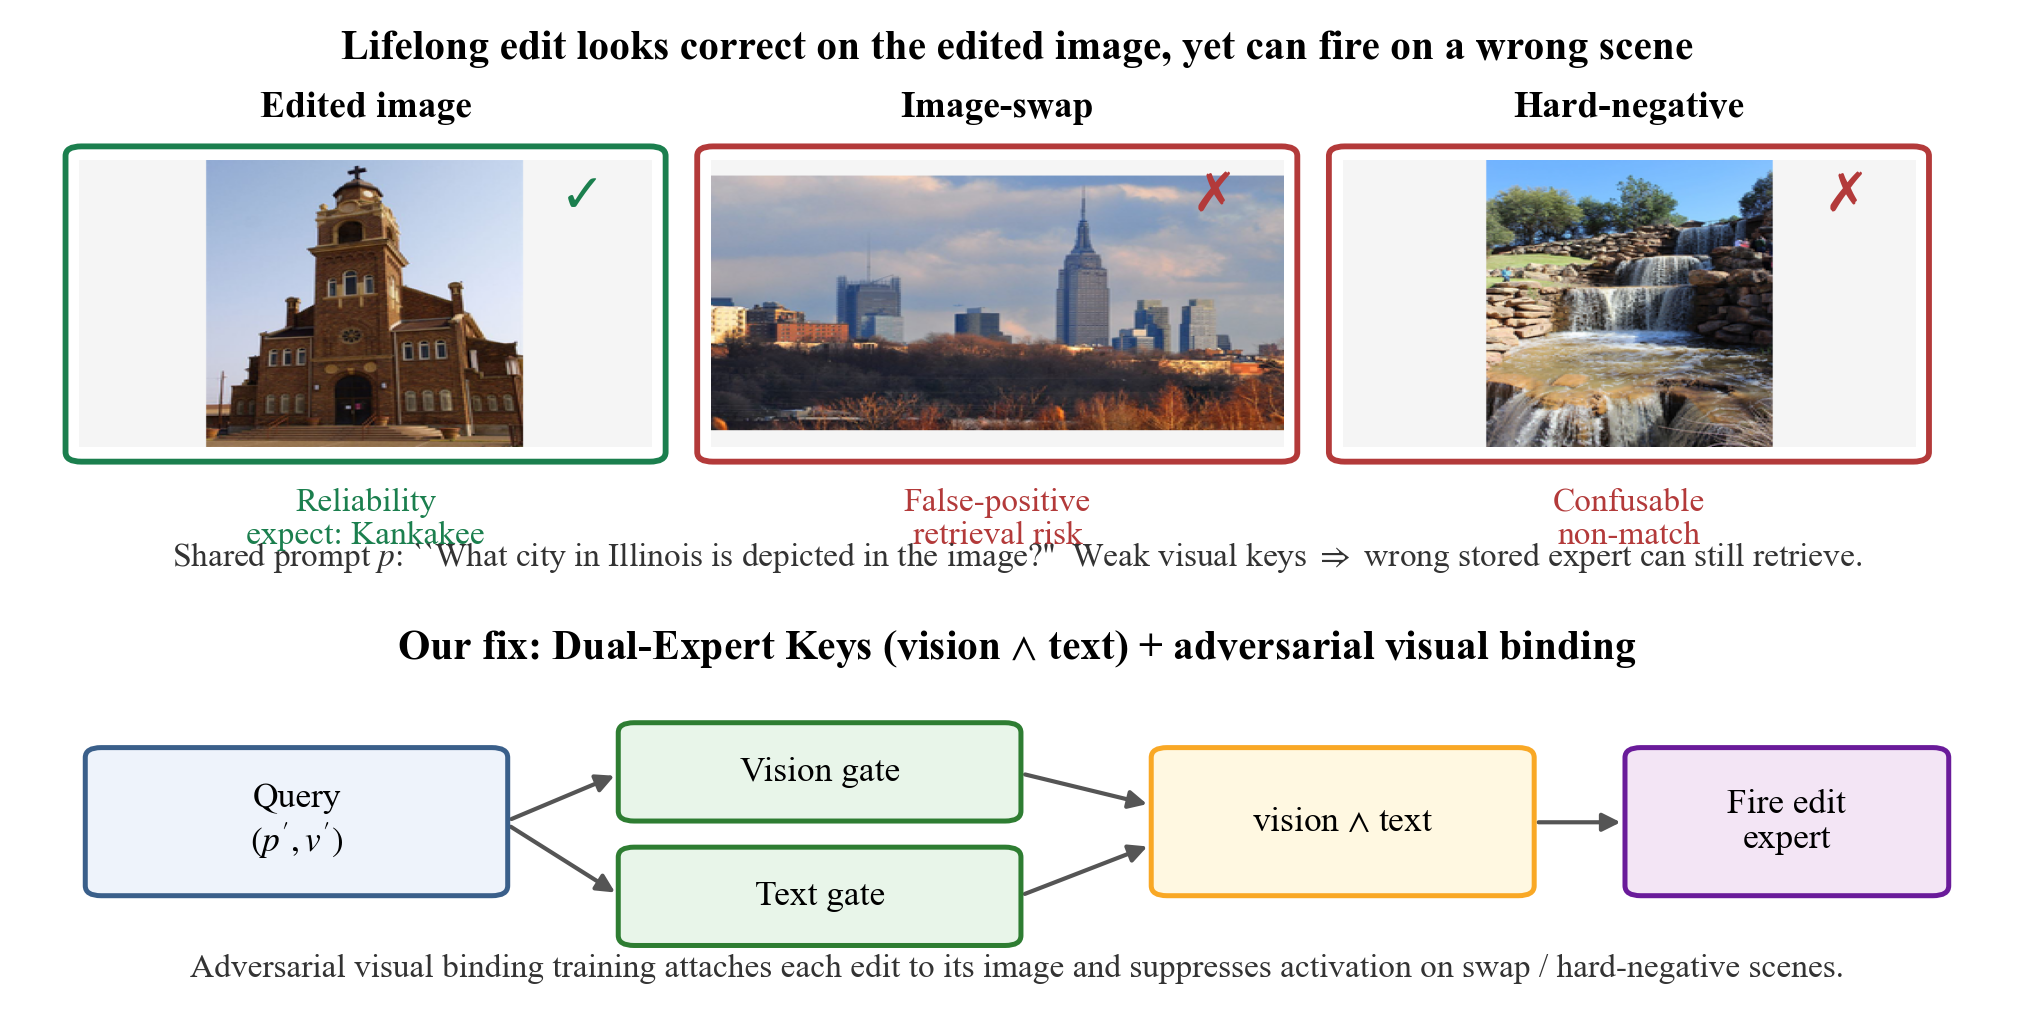
\includegraphics[width=\linewidth]{aaai/fig1_teaser.png}
\caption{Top: shared prompt with the edited image (reliability), an image-swap, and a hard-negative.
Bottom: Dual-Expert Keys fire an edit only when vision and text gates both pass; adversarial visual binding strengthens edit--image attachment under these probes.}
\label{fig:teaser}
\end{figure}

We find that this failure is usually not soft overwrite of the frozen base VLM.
On our adversarial grounding probes, routing logs show that a \emph{foreign} stored expert is retrieved for the swapped image---often at rates above 90\%.
We call this \emph{false-positive retrieval} (and \emph{false-cross} when we score it from expert identities): the visual key for edit $i$ is similar enough to query image $j\neq i$ that the wrong expert passes the retrieval threshold and injects the wrong fact.
This is a retrieval-safety problem, not merely an answer-quality problem.
Yet the metrics that dominate multimodal editing papers---reliability on the edited image, text/image generality, and locality on unrelated prompts~\citep{cheng2023mmedit,huang2024vlkeb,chen2025liveedit}---do not report which expert fired under image-swap or hard-negative probes.
Lifelong VLM editors such as LiveEdit already combine visual filtering with text routing~\citep{chen2025liveedit}, but those designs are optimized for Rel/Gen/Loc, not for measuring or blocking wrong-expert activation on adversarial images.
DualEdit studies \emph{where} to place modality-specific adapters for reliability--locality trade-offs~\citep{shi2025dualedit}; it does not address lifelong expert-pool leakage.
Weight-updating editors (Fine-tuning, MEND, SERAC)~\citep{mitchell2022mend,mitchell2022serac} can rewrite answers, but when the competing system is a growing expert memory they leave false-positive retrieval unmeasured.

\paragraph{Key insight.}
If leakage is dominated by wrong-expert selection, then improving only the binding of an edit to its own image is not enough: the retrieval rule itself must reject candidates unless \emph{both} modalities agree.
A vision-only gate can still admit a foreign edit whose visual key collides with the query; a text-only gate can still admit that edit when the prompt matches.
Requiring vision $\wedge$ text agreement turns retrieval into a dual check: the image must look like the edited scene \emph{and} the prompt must match the stored edit key.

\paragraph{Our approach.}
We study this failure on a lifelong MoE-style editor~\citep{chen2025liveedit} with BLIP-2~\citep{li2023blip2} as the frozen backbone---the setting where continuous expert pools make false-positive retrieval observable.
We introduce two complementary pieces.
(1)~\emph{Dual-Expert Keys (DEK)}: at inference, an expert may fire only when its visual gate and its prompt-key (text) gate both pass.
(2)~\emph{Adversarial visual binding training (AVBT)}: during editing, we attach each expert to its correct image and explicitly suppress fused expert activation on swap and hard-negative images.
DEK is the primary anti-leakage mechanism; AVBT stabilizes edit--image binding so the dual-gate is not fighting a weakly grounded expert.

\paragraph{Empirical preview.}
On VLKEB-based adversarial grounding probes~\citep{huang2024vlkeb}, Dual-Expert Keys cut the swap false-positive retrieval rate from $96\%$ to $46\%$ over five evaluation seeds while keeping reliability near $94\%$.
Standard Rel/Gen/Loc stay essentially on parity with the lifelong baseline.
Ablations show that binding training alone leaves false-cross near $96\%$; adding Dual-Expert Keys is what halves wrong-expert retrieval.
Under a matched long-form train/eval protocol, false-positive retrieval similarly falls from $88\%$ to $38\%$ with reliability held near $73\%$.
Against Fine-tuning, MEND-VL, and SERAC-VL on the same probes, our method is the one that keeps high reliability while directly reducing wrong-expert retrieval.
We emphasize the claim carefully: we target \emph{anti-leakage routing}, not token-level image-swap state of the art.

\paragraph{Contributions.}
This paper makes three contributions:
\begin{itemize}
    \item \textbf{Problem.} We characterize false-positive retrieval (false-cross) as a dominant visual grounding failure in lifelong multimodal editors under image-swap and hard-negative probes, and show that it is under-reported by Rel/Gen/Loc alone.
    \item \textbf{Method.} We propose Dual-Expert Keys, which require vision--text agreement at retrieval time, together with adversarial visual binding training that attaches edits to their images and suppresses adversarial activation.
    \item \textbf{Evidence.} On VLKEB grounding probes we show large false-positive cuts with reliability preserved, ablations that isolate Dual-Expert Keys as the FC mechanism, multi-seed stability, and comparisons to Fine-tuning, MEND-VL, and SERAC-VL.
\end{itemize}

Section~\ref{sec:related} situates the work; Section~\ref{sec:problem} formalizes probes and false-cross; Section~\ref{sec:method} presents AVBT and Dual-Expert Keys; Sections~\ref{sec:experiments}--\ref{sec:results} describe the experimental protocol and results; we close with limitations and conclusions.

\section{Related Work}
\label{sec:related}

\paragraph{Knowledge editing for language models.}
Modern LMs store large amounts of factual knowledge, but that knowledge can be wrong, outdated, or incomplete.
\emph{Model editing} aims to inject a local correction without full retraining and without broadly damaging unrelated behaviour~\citep{decao2021knowledgeeditor,yao2023editing}.
The literature is usually grouped into three families.
\emph{Locate-then-edit} methods first identify parameters associated with a fact and then rewrite them; ROME does this for single edits, and MEMIT scales the idea to many facts~\citep{meng2022rome,meng2023memit}.
\emph{Meta-learning} editors such as MEND train a hypernetwork to turn edit gradients into low-rank weight updates~\citep{mitchell2022mend}.
\emph{Memory / retrieval} editors keep the base model frozen and store edits externally: SERAC retrieves a counterfactual memory and routes through a scope classifier~\citep{mitchell2022serac}, GRACE maintains lifelong discrete key--value adaptors~\citep{hartvigsen2023grace}, and in-context editors such as IKE place edit demonstrations in the prompt~\citep{zheng2023ike}.
EasyEdit unifies many of these methods behind a common interface, which has made fair comparison easier~\citep{wang2024easyedit}.
Beyond single-fact reliability, later evaluation work asks whether an edit propagates consistently to related facts~\citep{cohen2024evaluating} and whether editors can handle long or diverse-format targets~\citep{jiang2025anyedit}.
AnyEdit is the closest long-form \emph{text} line: it edits chunk by chunk under an autoregressive locate-then-edit view~\citep{jiang2025anyedit}.
We cite it for that contribution, but it is not a competitor on VLKEB visual grounding: it has no image modality and no lifelong multimodal expert pool.

\paragraph{Multimodal knowledge editing and benchmarks.}
Editing vision--language models is harder than editing text-only LMs because the fact is tied to an image as well as a prompt~\citep{cheng2023mmedit}.
MMEdit established early multimodal reliability / generality / locality protocols for VQA- and caption-style edits~\citep{cheng2023mmedit}.
VLKEB improves visual quality by building edits from multimodal knowledge graphs and adds portability-oriented checks~\citep{huang2024vlkeb}.
More recent benchmarks push different axes: MC-MKE emphasizes modality consistency across fine-grained edit formats~\citep{zhang2025mcmke}, MMKE-Bench covers diverse visual semantics and free-form knowledge~\citep{du2025mmkebench}, and ComprehendEdit aggregates multiple tasks with generalization / preservation indices~\citep{ma2025comprehendedit}.
On the method side, DualEdit studies \emph{where} to edit: it updates text and vision at modality-sensitive layers and uses a gate to protect original behaviour~\citep{shi2025dualedit}.
That gating is about reliability--locality trade-offs under layer choice, not about blocking wrong-expert retrieval in a lifelong MoE pool.
Across this literature, success is still mostly reported as: the new answer appears on the edited (or rephrased) input, and unrelated inputs stay stable.
What is usually missing is an explicit account of \emph{which stored edit} fired when the prompt is held fixed and the image is swapped or made confusable.

\paragraph{Lifelong retrieval editors and visual keys.}
Lifelong editing requires many updates to coexist over time~\citep{hartvigsen2023grace,chen2025liveedit}.
LiveEdit is the closest system to our setting: it generates a low-rank MoE expert per edit, stores experts in a growing repository, and at inference uses hard visual filtering followed by soft text routing to fuse relevant experts into a frozen VLM such as BLIP-2~\citep{chen2025liveedit,li2023blip2}.
Related multimodal backbones used in editing studies include LLaVA and InstructBLIP~\citep{liu2023llava,dai2023instructblip}.
Because retrieval decides which residual is injected, routing quality becomes part of editing safety as the pool grows---an issue that sparse MoE selection has long faced in other domains~\citep{shazeer2017moe}.
Strong visual encoders can help in principle: CLIP-style vision--language similarity~\citep{radford2021clip} and DINOv2 features~\citep{oquab2024dinov2} often separate images well in offline probes.
But offline discrimination does not automatically transfer to \emph{edit retrieval} when the editor compresses vision into a few routing keys and scores them against a large lifelong pool.
Weight-updating multimodal adaptations of Fine-tuning, MEND, and SERAC remain important baselines~\citep{mitchell2022mend,mitchell2022serac,cheng2023mmedit}; they can change answers, yet they do not expose a growing expert identity that we can score for false-cross.

\paragraph{Positioning and distinction from close neighbours.}
Our focus is an under-measured lifelong multimodal failure: \emph{false-positive retrieval} (false-cross) under image-swap and hard-negative probes.
Dual-Expert Keys require vision $\wedge$ text agreement before an expert may fire; adversarial visual binding training attaches each edit to its image and suppresses activation on adversarial scenes.
This differs from DualEdit, which chooses modality-specific layers and a Rel/Loc gate~\citep{shi2025dualedit}, and from AnyEdit, which targets long-form text locate-then-edit~\citep{jiang2025anyedit}.
It also differs from benchmark papers that expand Rel/Gen/Loc, portability, or modality consistency without measuring wrong-expert retrieval rates~\citep{huang2024vlkeb,zhang2025mcmke,du2025mmkebench,ma2025comprehendedit}.
We use a LiveEdit-style lifelong MoE editor as the experimental \emph{testbed} because continuous expert pools make false-cross observable and actionable.
The scientific claim is not ``higher Rel/Gen/Loc than LiveEdit on the original leaderboard,'' but a diagnosis and mechanism for anti-leakage retrieval under adversarial images.

\section{Problem: Visual Grounding Leakage via False-Cross Retrieval}
\label{sec:problem}
% Define reliability vs image-swap / hard-negative probes.
% Define false-cross: retrieved expert belongs to a different edit than the queried image.
% Empirical pattern: high reliability, large swap-gap, FC often >90% under scalar visual keys.

Let an editor maintain a pool of stored edits (experts).
On a query (prompt, image), retrieval selects one or more experts to inject.
\emph{Reliability} measures accuracy on the edited image.
\emph{Image-swap} / \emph{hard-negative} probes reuse the edit prompt with a wrong or confusable image.
We define \emph{false-cross} as retrieving an expert whose edit identity does not match the queried image.
High false-cross means leakage is driven by wrong-expert selection, not only soft overwrite of the base model.

\section{Method}
\label{sec:method}

\subsection{Setting}
We consider a lifelong multimodal editor with a growing pool of edit experts.
At inference, retrieval decides which expert(s) inject into the model.

\subsection{Adversarial Visual Binding Training}
Adversarial visual binding training attaches each edit to its correct image evidence and lowers fused expert activation on swap and hard-negative images (hinge / contrastive binding loss).
It reshapes adversarial activation while preserving reliability on the correct image.
Binding training alone does not cut false-cross (remains near $96\%$ in our short probes).

\subsection{Dual-Expert Keys}
Dual-Expert Keys activate an expert only when the visual gate and the prompt-key (text) gate both pass.
This vision-and-text agreement rule is the primary mechanism for reducing false-cross (short: $96\%\!\rightarrow\!46\%$; fair long: $88\%\!\rightarrow\!38\%$).

\subsection{Negative Variants}
Neighbor mining and pool-buffer variants are reported as negative / appendix ablations; they are not our primary method.

\section{Experiments}
\label{sec:experiments}
% Protocol: BLIP2-OPT-2.7B; VLKEB grounding short/long; FC via routing logs.
% Comparisons: lifelong MoE baseline; FT-VL; MEND-VL; SERAC-VL.
% Ablation: baseline -> AVBT -> Dual-Expert Keys -> FX -> PB.
% Credibility: 5 eval seeds (short); fair matched long; significance where applicable.
% Metric order in tables: FC (lower better), reliability, then probe rates (state direction carefully).

\textbf{Backbone.} BLIP2-OPT-2.7B.
\textbf{Probes.} VLKEB grounding short (primary for July abstract); image-swap, hard-negative, reliability; false-cross from routing logs.
\textbf{Comparisons.} Lifelong MoE baseline; Fine-tuning; MEND-VL; SERAC-VL.
\textbf{Ablation.} Baseline $\rightarrow$ adversarial binding $\rightarrow$ Dual-Expert Keys $\rightarrow$ neighbor mining $\rightarrow$ pool buffer.
\textbf{Credibility.} Five evaluation seeds on short probes; optional matched long-form train/eval for the full PDF.

\section{Results}
\label{sec:results}
We report results on the short VLKEB grounding protocol ($dsn{=}100$, $sen{=}10$, seed $42$), which is our main evaluation setting.
Table~\ref{tab:standard-short} uses LiveEdit-style names: Rel, T-Gen (text rephrase), M-Gen (image rephrase), T-Loc, and M-Loc.
False-cross (FC) is the primary novelty metric (lower is better).

\begin{table}[t]
\centering
\begin{tabular}{lcccccc}
\toprule
Method & Rel$\uparrow$ & T-Gen$\uparrow$ & M-Gen$\uparrow$ & T-Loc$\uparrow$ & M-Loc$\uparrow$ & FC$\downarrow$ \\
\midrule
Lifelong baseline & 93.5\% & 94.3\% & 92.1\% & 100\% & 100\% & 96\% \\
AVBT (binding only) & 93.8\% & 94.5\% & 93.8\% & 100\% & 100\% & 96\% \\
Dual-Expert Keys (ours) & 93.7\% & 94.5\% & 92.0\% & 100\% & 100\% & \textbf{46\%} \\
\bottomrule
\end{tabular}
\caption{Short grounding: standard Rel/Gen/Loc are preserved; Dual-Expert Keys cut false-cross $96\%\!\rightarrow\!46\%$.}
\label{tab:standard-short}
\end{table}

Dual-Expert Keys match the lifelong baseline on Rel/T-Gen/M-Gen/T-Loc/M-Loc (within $\sim$0.2--0.3\,pp on Rel/T-Gen; M-Gen within $\sim$0.2\,pp of baseline).
Adversarial binding alone does not reduce FC (still $96\%$).
Adding Dual-Expert Keys halves false-cross while keeping the standard operating point.
This is the intended Results claim: \emph{parity on Rel/Gen/Loc, large gain on FC}.

% Placeholder for competitors / multi-seed / fair-long (fill before July 28 PDF).
% Sources: AAAI_ABLATION_TABLE.md, AAAI_COMPETITOR_TABLE_SHORT.md, AAAI_DEK_MULTISEED.md, AAAI_LONG_FAIR.md

\section{Limitations}
We claim anti-leakage routing (false-cross reduction with reliability held), not token-swap state of the art.
False-cross is defined for retrieval-pool editors and is not directly applicable to pure Fine-tuning / MEND / SERAC.
Results currently use a single backbone (BLIP2-OPT-2.7B).
Probe construction should be supported by a human audit of adversarial pairings.

\section{Conclusion}
False-cross retrieval is a concrete leakage mode in lifelong multimodal editing.
Dual-Expert Keys reduce wrong-expert retrieval by requiring vision--text agreement, with adversarial visual binding as training support, while preserving high reliability.

% Acknowledgments omitted for anonymous review.
% \section*{Acknowledgments}
% ...

\bibliography{aaai_refs}

\end{document}
